\documentclass[11pt,a4paper]{article}
\usepackage[margin=1in]{geometry}
\usepackage{booktabs}
\usepackage{graphicx}
\usepackage{microtype}
\usepackage{natbib}
\usepackage{url}
\usepackage[hidelinks]{hyperref}
\usepackage{caption}
\usepackage{subcaption}
\usepackage{placeins}

\graphicspath{{figures/}}
\setlength{\textfloatsep}{7pt}
\setlength{\floatsep}{7pt}
\setlength{\intextsep}{7pt}
\captionsetup{font=small}

\title{\vspace{-1.5em}Language Models, Embeddings, and Transfer to Sentiment Classification}
\author{TANG JIAYI / A0355738N}
\date{}

\begin{document}
\maketitle
\vspace{-2em}

\section{Introduction}
This work asks one question: how do model structure and embedding settings affect next-token
prediction, and do these differences transfer to downstream classification? I compare an
interpolated trigram model, RNN, LSTM, and causal Transformer on the same WikiText-2 token stream.
I then compare three LSTM embedding settings and use frozen LSTM and Transformer states for SST-2
sentiment classification. The main finding is that rankings depend on both training budget and
task. Across four 20-epoch seeds, the LSTM consistently has the best neural language-model
perplexity. Transformer mean pooling has the best average sentiment accuracy, but does not beat
LSTM mean pooling for every seed.

\section{Data \& Preprocessing}
I use WikiText-2 \citep{merity2017wikitext} from HuggingFace Datasets
\citep{lhoest2021datasets}. Text is lowercased, empty lines are removed, and \texttt{<eos>} is
added after each non-empty line. The vocabulary is built only from training data with minimum
frequency two. It contains 28,913 types; the train/validation/test streams contain
2,075,677/216,347/244,102 tokens. SST-2 \citep{socher2013sst,wang2018glue} uses 10,000 training,
2,000 validation, and 872 official-validation examples as test data. SST-2 is lowercased and
regex-tokenized into the WikiText vocabulary. Its OOV rates are 7.68\%, 7.37\%, and 6.92\% on the
three splits.
% Sources for all counts and OOV rates above: results_e20/part1/summary.json and results_e20/part3/summary.json.

\section{Models \& Experimental Setup}
The trigram model linearly interpolates trigram, bigram, unigram, and uniform probabilities, with
weights chosen on validation data. RNN and LSTM models use 100-dimensional embeddings, two
256-unit recurrent layers, dropout 0.3, and a linear output. The Transformer uses a
100-to-128 input projection, four heads, three layers, a 512-unit feed-forward block, learned
positions, dropout 0.1, and a causal mask. Neural models use context length 64, batch size 64,
AdamW with learning rate 0.001, and gradient clipping at 1.0. The main experiment trains for 20
epochs, and a supplementary experiment uses 8 epochs. The main results use seed 42. Seeds 1, 2,
and 3 repeat the 20-epoch experiment to assess stability (Table~\ref{tab:seeds}). The 8-epoch
experiment uses seed 42 only. The best validation checkpoint is tested once.
Perplexity is the exponential of mean non-padding token cross-entropy. Experiments ran on a
Colab Tesla T4 with Python 3.13.15 and PyTorch 2.11.0.
% Sources: config.yaml; results_e20/part1/summary.json.

For generation, all models use temperature 0.8, top-$k$ 40, 30 new tokens, five fixed prompts, and
matched seeds. Timings synchronize the GPU, and throughput uses the same test workload. Part II
keeps the LSTM fixed apart from its input table: random trainable embeddings, corpus-trained
Skip-gram via gensim \citep{rehurek2010gensim}, or public 100d GloVe
\citep{pennington2014glove}. The two imported tables are frozen. Part III freezes each language
model and fits StandardScaler plus logistic regression, selecting $C\in\{0.01,0.1,1,10\}$ only
on validation data.

The complete code and reproduction instructions are available at
\url{https://github.com/Ala-Tang/nlp-language-models-dsa4213}.

\section{Part I: Language Models}
\begin{table}[t]
\centering
\small
\caption{Main 20-epoch language-model results. Lower perplexity is better.}
\begin{tabular}{lrrrr}
\toprule
Model & Test PPL & Parameters & Train (s) & Tokens/s \\
\midrule
Trigram & 264.65 & 0 & 26.36 & 351,650 \\
RNN & 175.89 & 10,545,173 & 843.26 & 191,976 \\
LSTM & \textbf{154.73} & 11,214,869 & 920.69 & 166,892 \\
Transformer & 163.06 & 7,237,013 & 637.81 & 290,536 \\
\bottomrule
\end{tabular}
% Source: results_e20/part1/summary.json.
\label{tab:part1}
\end{table}

We observe that the LSTM has the lowest test perplexity (154.73), followed by the Transformer
(163.06) and RNN (175.89). The Transformer is smaller and faster than both recurrent models, so
the LSTM quality gain costs more parameters and time. A possible explanation is that LSTM gating
helps on this training budget, but architecture is confounded with parameter count.

\begin{figure}[t]
\centering
\begin{subfigure}{0.49\linewidth}
  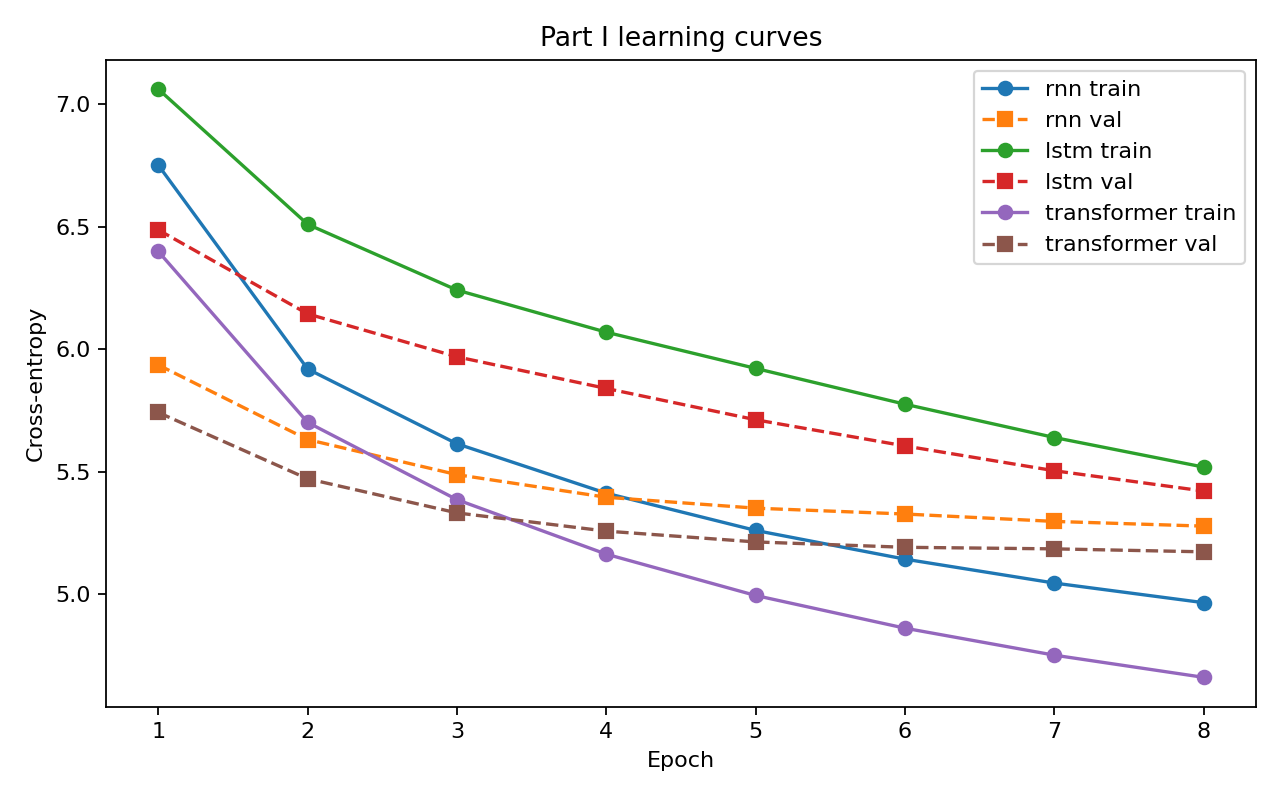
\includegraphics[width=\linewidth]{part1_e8_loss_curves.png}
  \caption{Eight epochs.}
\end{subfigure}
\begin{subfigure}{0.49\linewidth}
  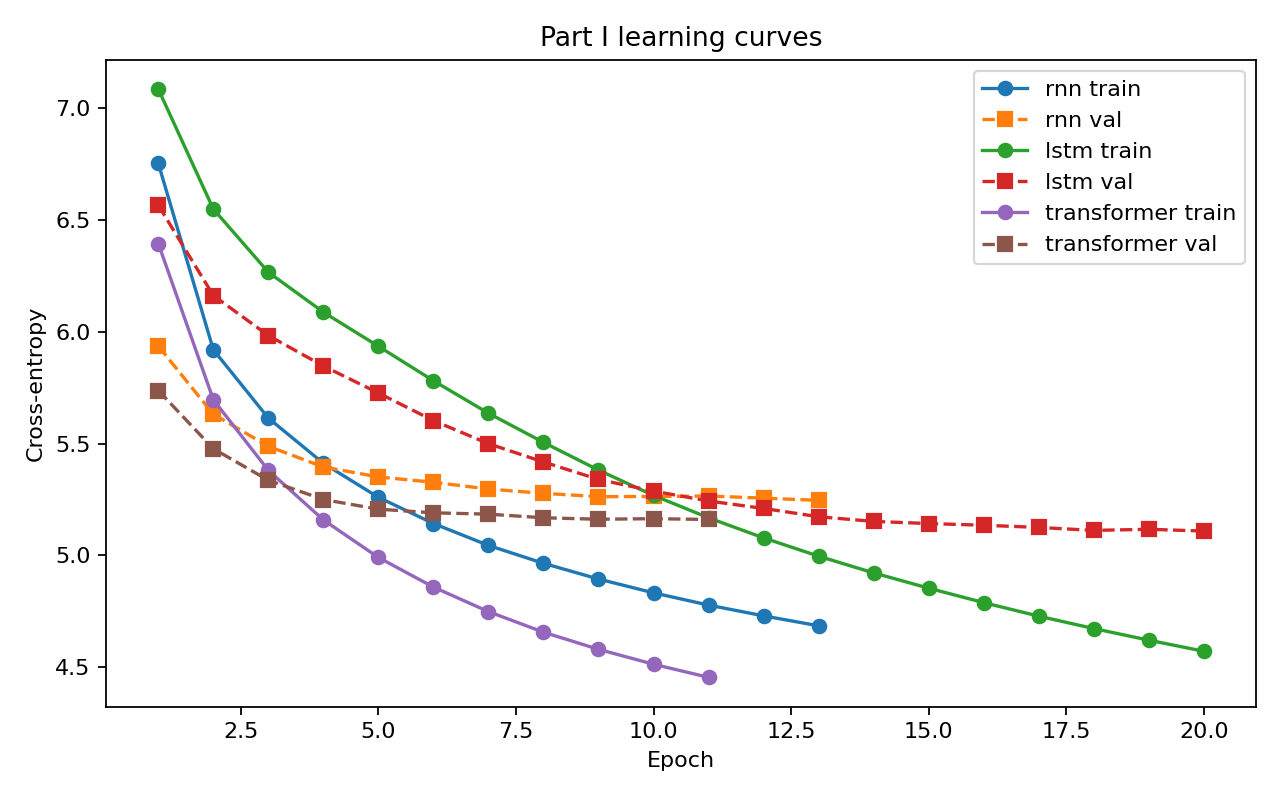
\includegraphics[width=\linewidth]{part1_e20_loss_curves.png}
  \caption{Twenty epochs.}
\end{subfigure}
\caption{Part I learning curves under two training budgets.}
% Sources: results_e8/part1/loss_curves.png and results_e20/part1/loss_curves.png.
\label{fig:part1curves}
\end{figure}

The ranking changes with budget (Table~\ref{tab:budget}). At 20 epochs, validation loss is best
for LSTM at epoch 20 (5.109), Transformer at epoch 11 (5.161), and RNN at epoch 13 (5.246).
RNN and Transformer then continue reducing training loss without improving their best validation
loss. Their final validation-minus-training gaps are 0.817 and 1.062, versus 0.537 for LSTM.
We observe possible overfitting for the first two. In contrast, the LSTM still improves at epoch
20, so it may not be fully converged.
% Sources: results_e20/part1/log.txt and results_e20/part1/summary.json.

\begin{table}[t]
\centering
\small
\caption{Test perplexity ranking changes with training budget.}
\begin{tabular}{p{0.13\linewidth}p{0.78\linewidth}}
\toprule
Budget & Ranking from lower to higher perplexity \\
\midrule
8 epochs & Transformer 164.55 $<$ RNN 180.65 $<$ LSTM 211.29 $<$ trigram 264.65 \\
20 epochs & LSTM 154.73 $<$ Transformer 163.06 $<$ RNN 175.89 $<$ trigram 264.65 \\
\bottomrule
\end{tabular}
% Sources: results_e8/part1/summary.json and results_e20/part1/summary.json.
\label{tab:budget}
\end{table}

Generated text supports only a limited qualitative comparison. The trigram continuation for
``the meaning of life'' repeats \texttt{= = = =}, while neural outputs form longer local phrases.
However, topic consistency remains weak: the 20-epoch Transformer changes ``once upon a time''
into a hurricane entry. These examples show local fluency differences, not general quality.
% Source: results_e20/part1/generations.md.

\section{Part II: Embedding Variants}
\begin{table}[t]
\centering
\small
\caption{Twenty-epoch LSTM embedding comparison. Gap is final validation minus training loss.}
\begin{tabular}{lrrrr}
\toprule
Embedding & Test PPL & Best val & Final gap & LM train (s) \\
\midrule
Random, trainable & 154.73 & 5.109 & 0.537 & 920.69 \\
Word2Vec, frozen & \textbf{146.52} & \textbf{5.048} & 0.500 & 907.08 \\
GloVe, frozen & 147.12 & 5.050 & \textbf{0.368} & 904.14 \\
\bottomrule
\end{tabular}
% Sources: results_e20/part2/summary.json, results_e20/part2/log.txt, and results_e20/part1/log.txt.
\label{tab:part2}
\end{table}

Word2Vec covers 28,912 of 28,913 types (99.997\%) and takes 65.00 seconds to train. GloVe covers
27,809 types (96.182\%). Both frozen variants pass the exact freeze check. We observe that both
beat the trainable random table for seed 42, while Word2Vec and GloVe are close. A possible
explanation is that freezing regularizes the large input table. Word2Vec is slightly better in
the seed-42 run, but the two frozen settings trade places across the four seeds. Their mean
gap is 0.54, below the combined sample standard deviation of 2.63 (Table~\ref{tab:seeds}), so
this experiment cannot distinguish them. External data does not provide a reliable additional benefit here.
% Sources: results_e20/part2/coverage.json, results_e20/part2/summary.json, and results_e20/part2/log.txt.

For seed 42, budget again matters: at eight epochs the ranking is Word2Vec 180.89, random 211.29, and GloVe
229.73, while at twenty epochs it is Word2Vec 146.52, GloVe 147.12, and random 154.73. GloVe
starts slowly but nearly catches Word2Vec. Its smaller final train--validation gap is consistent
with stronger regularization, although this is a hypothesis rather than a controlled test.
% Sources: results_e8/part2/summary.json and results_e20/part2/summary.json.

\begin{figure}[t]
\centering
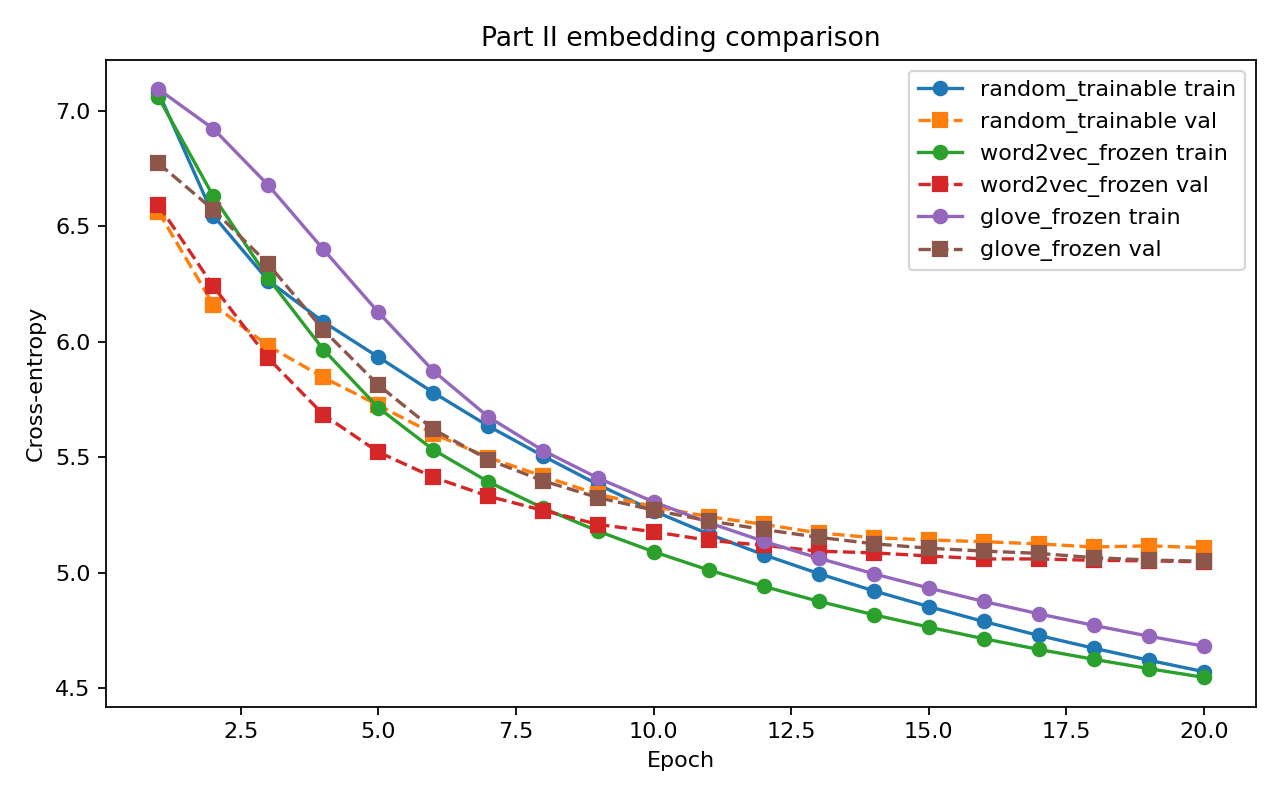
\includegraphics[width=0.82\linewidth]{part2_e20_loss_curves.png}
\caption{Part II training and validation losses for the three embedding settings.}
% Source: results_e20/part2/loss_curves.png.
\label{fig:part2curves}
\end{figure}

Figure~\ref{fig:part2curves} shows smooth loss reduction for all settings, without large spikes.
GloVe improves more slowly in the first three epochs, while Word2Vec reaches a low validation loss
earlier. By epoch 20 their validation losses are close (5.050 and 5.048). For the prompt ``the
meaning of life'', the random setting repeats WikiText heading markers
\texttt{<eos> = = reception = =}; Word2Vec also produces heading markers but then forms a more
locally fluent phrase about the 1960s. GloVe repeats ``never never'' and has weaker grammar
(``they cannot really that''). We observe different local errors, but five prompts are too few
to establish a general generation ranking.
% Sources: results_e20/part2/log.txt and results_e20/part2/generations.md.

\section{Part III: Downstream Representations}
For each sentence, I keep at most the first 64 lowercased regex tokens and pad shorter inputs.
Both models use the sequence of last-layer hidden states. Mean representations multiply each
state by the non-padding mask, sum over positions, and divide by the number of real tokens.
The LSTM last-state control selects the last-layer state at the final non-padding position.
% Sources: data.py (ClassificationDataset) and part3.py (extract_representations).

\begin{table}[t]
\centering
\small
\caption{SST-2 test results from frozen language-model representations.}
\begin{tabular}{lrrr}
\toprule
Representation & Selected $C$ & Accuracy & Macro-F1 \\
\midrule
LSTM mean & 0.01 & 0.6456 & 0.6442 \\
Transformer mean & 0.01 & \textbf{0.6640} & \textbf{0.6625} \\
LSTM last state & 0.01 & 0.6261 & 0.6234 \\
Majority class & -- & 0.5092 & -- \\
\bottomrule
\end{tabular}
% Sources: results_e20/part3/summary.json and results_e20/part3/errors.csv.
\label{tab:part3}
\end{table}

\begin{table}[ht]
\centering
\footnotesize
\caption{Four-seed 20-epoch results (mean $\pm$ sample standard deviation).}
\begin{tabular}{p{0.07\linewidth}p{0.35\linewidth}p{0.48\linewidth}}
\toprule
Part & Model or representation & Metric \\
\midrule
I & Trigram & 264.65 PPL (deterministic) \\
I & RNN & $177.04 \pm 1.38$ PPL \\
I & LSTM & $\mathbf{154.14 \pm 1.36}$ PPL \\
I & Transformer & $162.46 \pm 0.46$ PPL \\
II & Random / Word2Vec / GloVe & $154.14\pm1.36$ / $146.60\pm0.57$ / $146.05\pm2.57$ PPL \\
III & LSTM mean & Acc.\ $0.6345\pm0.0111$; F1 $0.6336\pm0.0105$ \\
III & Transformer mean & Acc.\ $\mathbf{0.6416\pm0.0174}$; F1 $\mathbf{0.6405\pm0.0173}$ \\
III & LSTM last & Acc.\ $0.6095\pm0.0129$; F1 $0.6066\pm0.0123$ \\
\bottomrule
\end{tabular}
% Sources: results_e20/{part1,part2,part3}/summary.json and corresponding summary.json files
% in results_seed1, results_seed2, and results_seed3; aggregated by aggregate_seeds.py.
\label{tab:seeds}
\end{table}

For seed 42, both masked-mean representations beat the LSTM last state, and Transformer mean has
the highest accuracy. In that run the rankings disagree: the LSTM has lower perplexity than the
Transformer (154.73 versus 163.06) but lower accuracy (0.6456 versus 0.6640). Across four seeds,
the Part I ranking is identical. The mean LSTM--Transformer perplexity gap is 8.31, larger than
their combined sample standard deviation of 1.44, so the perplexity advantage is stable. The mean
accuracy gap between Transformer mean and LSTM mean is only 0.0072, below their combined sample
standard deviation of 0.0206, and seed 2 reverses their order. The perplexity advantage therefore
does not reliably become a classification advantage. Both mean representations are more
consistently above the LSTM last state. In the seed-42 eight-epoch run, the Transformer ranks
first on both perplexity and classification, but that comparison uses one seed. Domain shift from
WikiText to reviews and the 6.92\% test OOV rate remain plausible factors; these results do not
isolate them.
% Sources: results_e20/part3/summary.json, results_e8/part1/summary.json,
% results_e8/part3/summary.json, and analysis/multiseed_summary.json.

The test set contains 428 negative and 444 positive examples, so always predicting the positive
majority gives 0.5092 accuracy. All learned representations are well above this weak baseline.
% Source: results_e20/part3/errors.csv.

Manual error inspection shows recurring surface patterns. Mixed statements such as ``nothing
outstanding ... but ... good enough'' split the two mean representations. Sarcasm or indirect
criticism such as ``Holden Caulfield did it better'' and rhetorical questions are also difficult.
Some positive comparisons are missed by LSTM mean but found by Transformer mean. These categories
describe seed-42 examples; they do not establish causal failure modes.
% Source: results_e20/part3/errors.csv.

\FloatBarrier

\section{Limitations \& Lessons}
The LSTM may not be fully converged at 20 epochs, so its final ranking can still change. All neural
models are small, and architecture comparisons are confounded by parameter count. WikiText and
SST-2 have different domains, while SST-2 still contains OOV tokens. T4 kernels can be
nondeterministic: the first eight epochs of the seed-42 8-epoch run and the seed-42 20-epoch
run match exactly for RNN losses only at the four decimal places stored in the logs, while the
LSTM and Transformer values differ slightly. Four seeds give only a limited view of
variance. For seed 42, all three classifiers select $C=0.01$, the lower search boundary. Across
seeds, selected values vary: LSTM mean uses 0.01--1, Transformer mean 0.01--0.1, and LSTM last
reaches the upper boundary 10 for seed 3. The search range may therefore be too narrow. The main
lesson is to report training budget and downstream evaluation together, because neither short-run
perplexity nor one embedding assumption gives a stable overall ranking.
% Source: analysis/multiseed_summary.json.

\section{AI/Tool Use Statement}
Cursor, an AI programming assistant, was used to write the code and draft the report. Claude was
used for experiment planning, interpretation of the results, and review. The experimental design
was proposed with this assistance and reviewed and approved by the author. The author ran the
experiments, checked the fairness of comparisons, and verified the results. The drafted report
was then reviewed and revised by the author.

\bibliographystyle{plainnat}
\bibliography{references}

\appendix
\section{Per-seed Results and Additional Generations}
The four-seed Part I PPL values are: RNN 175.89, 177.28, 178.88, 176.09; LSTM 154.73, 153.40,
155.75, 152.69; and Transformer 163.06, 162.21, 162.02, 162.55, ordered as seeds 42, 1, 2, 3.
Part II Word2Vec values are 146.52, 147.31, 145.91, 146.64, while GloVe values are 147.12,
143.20, 144.84, 149.06. Full accuracy, macro-F1, and selected-$C$ values are provided by
\texttt{analysis/multiseed\_summary.json}.
% Sources: analysis/multiseed_summary.json and analysis/multiseed_summary.md.

For ``in the beginning'', Word2Vec continues with ``of the 20th century'', whereas GloVe begins
``of the 19th century'' before losing semantic consistency. For ``the United States'', all three
settings produce locally plausible Wikipedia-like text but mix unrelated entities and events.
These additional examples reinforce the limited qualitative conclusion in Part II.
% Source: results_e20/part2/generations.md.

\end{document}
